\section{Auswertung}
\label{sec:Auswertung}
\subsection{Geiger-Müller Kennlinie}
Zunächst wird die Geiger Müller Kennlienie aus den Messwerten 
Der Zählrate pro Minute in Abhängigkeit von Der Detektorspannung
dargestellt. Die Kennlienie ist in \autoref{fig:10} dargestellt. 
Daas Geiger-Müller Plateu ist gut zu erkennen. Es Fängt bei 
$340\unit{\volt}$ an und endet nach $640\unit{\volt}$, da die Anzahl 
der Impulse pro Minute sich in dem Schritt von $640$ auf $660\unit{\volt}$
von vorher 3594 auf 7244 mehr als verdoppeln. Die Messwerte sind 
\autoref{tab:10} zu entnehmen. 

\begin{table}[H]
    \centering
    \caption{Detektorspannung zu Strom und Zählrade pro minute des Zählers.}
    \label{tab:10}
    \begin{tblr}{
            colspec = {S S S S S S},
            row{1} = {guard, mode = math},
        }
        \toprule
        U_D \, \unit{\volt}& I \, \unit{\ampere}& N \, \unit{1\per\second} & U_D \, \unit{\volt}& I \, \unit{\ampere}& N \, \unit{1\per\second}\\
        \midrule
        300  &   0.2  &   829   &  500  &   0.2  &   3531\\
        320  &   0.2  &   3482  &  520  &   0.2  &   3547\\
        340  &   0.2  &   3561  &  540  &   0.2  &   3572\\
        360  &   0.2  &   3456  &  560  &   0.2  &   3632\\
        380  &   0.2  &   3492  &  580  &   0.4  &   3518\\
        400  &   0.2  &   3537  &  600  &   0.4  &   3538\\
        420  &   0.2  &   3527  &  620  &   0.4  &   3528\\
        440  &   0.2  &   3646  &  640  &   0.4  &   3594\\
        460  &   0.2  &   3591  &  660  &   0.4  &   7244\\
        480  &   0.2  &   3468  &       &        &       \\
        \bottomrule 
    \end{tblr}
\end{table}
\begin{figure}
    \centering
    \caption{Geiger-Müller Kennlinie}
    \label{fig:10}
    \includegraphics{plot1.pdf}
\end{figure}
Als Arbeitsspannung, mit welcher wir im nächsten Teil weiterarbeiten
haben wir $560\unit{\volt}$ gewählt. Dieser Wert is in \autoref{fig:10} 
markiert, er befindet sich ungefähr bei Zwei Drittel des Plateaus, was sich 
der Literatur nach als Bewährter Messbereich bewährt hat. Durch die Folgende
Formel, welche auch in der \autoref{sec:Theorie} erwähnt wurde, wird 
die Steigung des Plateaus bestimmt. Diese Steigung ist ein Maß
für die güte des Plateaus. Eine geringe Steigung bedeutet das Pateau 
ist gut. 
\begin{equation}
    s = \frac{z\left(U_\text{A} + 50\unit{\volt}\right) - z\left(U_\text{A} - 50\unit{\volt}\right)}{z \cdot U_\text{A}} \cdot \frac{100\%}{100\unit{\volt}}
\end{equation}

Neben der Zählrate $N$ wurde auch der Strom $I$ in Abhängigkeit 
Der Spaannung aufgenommen. Aus dem zusammenhang in Verbindung 
mit der Zählrate kann durch die Formel 
\begin{equation}
    Q = \frac{I}{N \cdot \text{e}}
\end{equation}
Die Anzahl der Ladungsträger bestimmt werden. In \autoref{fig:11} ist die 
Ladungsträger-Anzahl gegen die Betriebsspannung $U_A$ aufgetragen. Jedoch ist 
zu erkennen, dass die Werte kaum aussagekräftig sind, da der Stom 
in $0.2 \unit{\ampere}$ schritten abgelesen wurde und der Strom 
nie $0.4 \unit{\ampere}$ überschritt.
\begin{figure}[H]
    \centering
    \caption{Anzahl der Ladungsträger abhängig von der Betriebsspannung}
    \label{fig:11}
    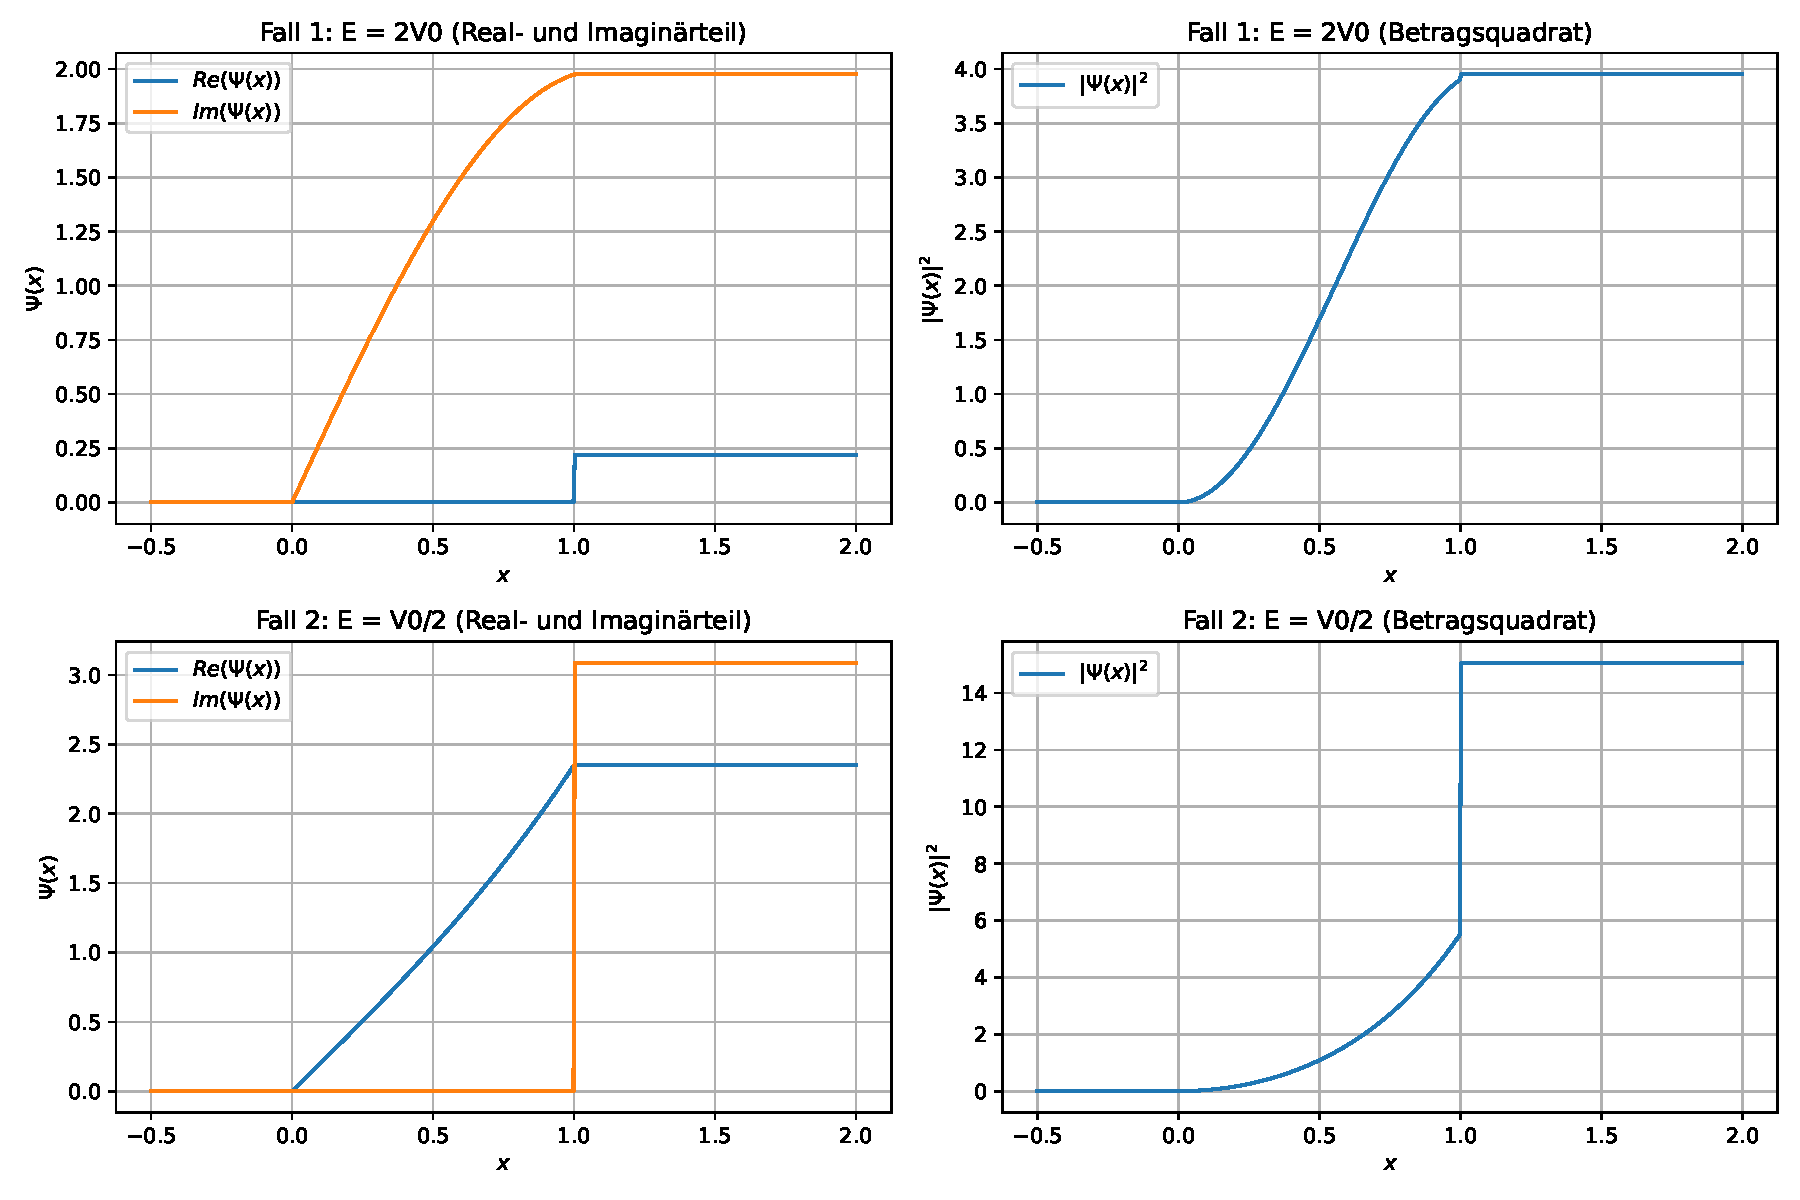
\includegraphics{plot2.pdf}
\end{figure}

\subsection{Bestimmung der Todzeit}
Die Todzeit wird zuerst mit der Zwei Quelen Methode bestimmt. Es 
werden die Zählraten zweier Quellen zunächst getrennt gemessen und 
dann die Zählrate über $200 \unit{\second}$ von beiden Quelllen zusammen. Dies geschieht bei der 
Arbeitsspannung von $U = 560 \unit{\volt}$. Die Todzeit errechnet sich dann 
durch Folgende Formel.
\begin{equation}
    \tau = \frac{N_\text{1} + N_\text{2} - N_\text{12}}{N_\text{12}^2  N_\text{2}^2 - N_\text{2}^2}
\end{equation}
Mit den Werten $N_\text{1} = 11936, N_\text{2} = 15383 $und$ N_\text{12} = 27556$ ergibt sich eine 
experimentelle Todzeit bei Messung mit der Zwei Quellen Methode von 
\begin{equation}
    \tau = \qty{-6.23e-7}{\second} 
\end{equation}

Bei der Bestimmung der Todzeit am Osziloskopbild wird der Abstand von zwei Impulsen am Osziloskop 
abgelesen und als todzeit gewertet. Durch ablesen ergibt sich eine Todzeit 
von $\tau = 150 \unit{\micro\second}$
\begin{figure}[H]
    \centering
    \caption{Osziloskopbild zur bestimmung der Todzeit}
    \label{fig:12}
    \includegraphics[width=0.65\textwidth]{Bilder/totzeit.jpg}
\end{figure} 

